\chapter{Communication Technologies}\label{Communications}

% Add Social Media?

\newenvironment{ucclist}[1]
{
	\begin{mdframed}[nobreak=true]
	\subsection{#1}
	\begin{mdframed}
		Address:  <\href{mailto:#1@ucc.asn.au}{#1@ucc.asn.au}>
	\end{mdframed}
	\begin{mdframed}
		Subscribe:  \small{\url{http://lists.ucc.asn.au/mailman/listinfo/#1}}
	\end{mdframed}


	
}{\end{mdframed}}
\section{Social Media}

Dragging itself kicking and screaming into the 21st Century, UCC has managed to set up a social media presence in something called the "cloud".

\begin{itemize}
\item UCC Facebook Group: \url{https://www.facebook.com/groups/universitycomputerclub/}
\item UCC Steam Group: \url{http://steamcommunity.com/groups/UCC}
\item UCC Status Twitter Account \tiny{(used mainly to tell everyone things are broken)}: \url{https://twitter.com/ucc_status}
\item GitHub: \url{https://github.com/ucc}

\end{itemize}

\section{Mailing Lists}

UCC often uses email for communication. There are various lists that you can sign up for at \url{http://lists.ucc.asn.au}. The most popular lists are \texttt{ucc-announce@} for announcements and \texttt{ucc@} for general discussion.


If you are interested in technology, join the \texttt{tech@} list. If you want to be kept up to date with management of the club, join \texttt{committee@}.



\section{IRC}

Without a doubt, the easiest way to waste time in or out of UCC 
is chatting on our Internet Relay Chat (IRC) server. 

You'll get to chat with some of the older members of the club who 
may not even be in Perth. Some of these old guard may seem a 
little grumpy or intimidating at first, but give them a chance, they 
are gold mines for information about the club and all things tech! 
We also have members from CASSA and ComSSA, clubs at other WA unis. 

You can connect with an IRC client to \texttt{irc://irc.ucc.asn.au:6667} 
and join the channel \texttt{\#ucc}, or with a web browser go to 
\url{http://irc.ucc.asn.au}

%\begin{figure}[H]
%	\centering
%	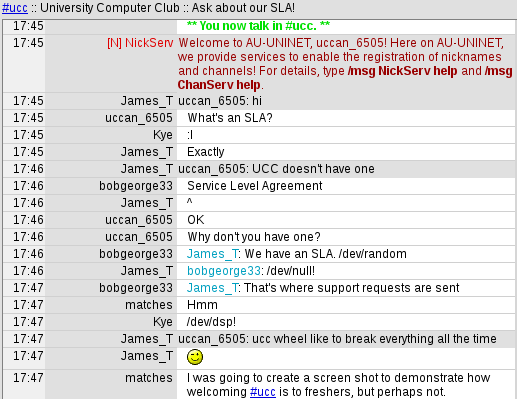
\includegraphics[width=0.99\textwidth]{figures/webirc2.png}
%	\caption{What normally happens when a Fresher joins IRC}
%	\label{webirc.jpg}
%\end{figure}

%IRC produces some incredible quotes. You can see these at \url{http://zanchey.ucc.asn.au/qdb/}.

%I didn't say they were wise or funny, just incredible.


